

\tikzset{every picture/.style={line width=0.75pt}} %set default line width to 0.75pt        

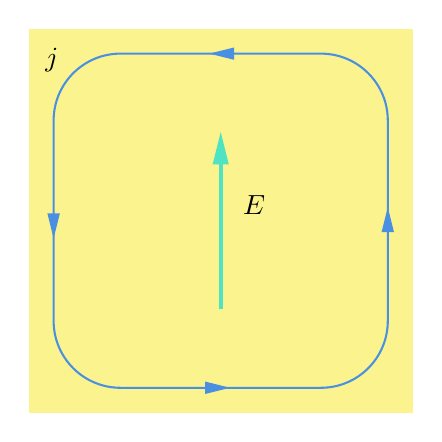
\begin{tikzpicture}[x=0.75pt,y=0.75pt,yscale=-1,xscale=1]
%uncomment if require: \path (0,300); %set diagram left start at 0, and has height of 300

%Shape: Square [id:dp8110413682744386] 
\draw  [draw opacity=0][fill={rgb, 255:red, 248; green, 231; blue, 28 }  ,fill opacity=0.5 ] (196,90) -- (381,90) -- (381,275) -- (196,275) -- cycle ;
%Straight Lines [id:da548073548119657] 
\draw [color={rgb, 255:red, 80; green, 227; blue, 194 }  ,draw opacity=1 ][line width=1.5]    (288.5,225.25) -- (288.5,143.75) ;
\draw [shift={(288.5,139.75)}, rotate = 90] [fill={rgb, 255:red, 80; green, 227; blue, 194 }  ,fill opacity=1 ][line width=0.08]  [draw opacity=0] (15.6,-3.9) -- (0,0) -- (15.6,3.9) -- cycle    ;
%Rounded Rect [id:dp9220949409043817] 
\draw  [color={rgb, 255:red, 74; green, 144; blue, 226 }  ,draw opacity=1 ] (208,134.2) .. controls (208,116.42) and (222.42,102) .. (240.2,102) -- (336.8,102) .. controls (354.58,102) and (369,116.42) .. (369,134.2) -- (369,230.8) .. controls (369,248.58) and (354.58,263) .. (336.8,263) -- (240.2,263) .. controls (222.42,263) and (208,248.58) .. (208,230.8) -- cycle ;
%Straight Lines [id:da6028379127452343] 
\draw [color={rgb, 255:red, 74; green, 144; blue, 226 }  ,draw opacity=1 ]   (290,102) -- (285,102) ;
\draw [shift={(283,102)}, rotate = 360] [fill={rgb, 255:red, 74; green, 144; blue, 226 }  ,fill opacity=1 ][line width=0.08]  [draw opacity=0] (12,-3) -- (0,0) -- (12,3) -- cycle    ;
%Straight Lines [id:da16991469576308726] 
\draw [color={rgb, 255:red, 74; green, 144; blue, 226 }  ,draw opacity=1 ]   (208,182) -- (208,189) ;
\draw [shift={(208,191)}, rotate = 270] [fill={rgb, 255:red, 74; green, 144; blue, 226 }  ,fill opacity=1 ][line width=0.08]  [draw opacity=0] (12,-3) -- (0,0) -- (12,3) -- cycle    ;
%Straight Lines [id:da0056621577609063944] 
\draw [color={rgb, 255:red, 74; green, 144; blue, 226 }  ,draw opacity=1 ]   (293,263) ;
\draw [shift={(293,263)}, rotate = 180] [fill={rgb, 255:red, 74; green, 144; blue, 226 }  ,fill opacity=1 ][line width=0.08]  [draw opacity=0] (12,-3) -- (0,0) -- (12,3) -- cycle    ;
%Straight Lines [id:da45045547035779476] 
\draw [color={rgb, 255:red, 74; green, 144; blue, 226 }  ,draw opacity=1 ]   (369,188) -- (369,178) ;
\draw [shift={(369,176)}, rotate = 90] [fill={rgb, 255:red, 74; green, 144; blue, 226 }  ,fill opacity=1 ][line width=0.08]  [draw opacity=0] (12,-3) -- (0,0) -- (12,3) -- cycle    ;

% Text Node
\draw (297.75,169) node [anchor=north west][inner sep=0.75pt]    {$\boldsymbol{E}$};
% Text Node
\draw (202.5,112.5) node [anchor=south west] [inner sep=0.75pt]    {$\boldsymbol{j}$};


\end{tikzpicture}
